\documentclass[a4paper,12pt]{article}

\usepackage{hyperref}
\usepackage{graphicx}

\title{PCUTL - Module 2:\\ Pedagogic Models, Inclusive Teaching and Technology}
\author{Vincent Knight}
\date{\today}

\begin{document}

\maketitle

%The ILOs for this portfolio are:
%\begin{enumerate}
%\item Describe key pedagogical models relevant to teaching and supporting learning in their subject discipline, and relate them to their own practice.
%\item Plan and run teaching sessions that explicitly considers contact and non-contact learning support and account for individual differences between learners. Critique the use of technology to enhance learning during contact and non-contact time learning.
%\item Draw on multi-source data to evaluate the impact of their teaching and/or support for learning on the breadth / diversity of students’ learning, and plan modifications accordingly.
%\item Identify further professional development needs in relation to teaching and/or supporting student learning.
%\end{enumerate}
%
%The program values for this portfolio are:
%
%\begin{enumerate}
%    \item An understanding of how students learn
%    \item A commitment to reflection and evaluation and consequent improvement of professional practice.
%    \item A respect for individual learners and for their development and empowerment, no matter what their circumstances.
%    \item A commitment to scholarship in teaching, both generally and within their own discipline.
%    \item A commitment to the development of learning communities, including students, teachers and those engaged in learning support.
%    \item A commitment to encouraging participation in higher education with respect to the issues of equality and diversity. In this regard, professional practice should be informed by equal opportunities legislation, policy and best practice.
%\end{enumerate}

R. L. Moore (1882-1974):
\begin{center}
    ``The student is taught the best who is told the least''
\end{center}

This portfolio contains material relevant to my Module 2 submission of pcutl. In this portfolio I have explored at a more detailed level various aspects of my teaching and my students' learning:

\begin{itemize}
    \item Thanks to an analysis of feedback received from students I have evaluated my effectiveness as a teacher;
    \item I have carefully explored issues of inclusivity and diversity through interactions with my peers and careful exploration of the literature. I will describe in this document the potential for various technological tools available to improve my consideration of these issues;
    \item Through a detailed review of the literature I have evaluated in detail various pedagogic models and I will in this document describe a particular pedagogy that I feel is appropriate to myself and my students.
\end{itemize}

\section{Analysis of feedback from previously taught module}\label{Analysis}

The  feedback was given via an online questionnaire and was mainly concerned with my use and in particular the student engagement with technology in the class (I already use my own website, videos, social networks and various other interactive tools in my teaching). The general consensus of the student feedback is positive. 70\% of my students watched various videos made available to them prior to lectures and 60\% of my students viewed my posts on Google Plus (a social network). I collected similar encouraging statistics with regards to the use of my own website for hosting notes, the use of an open source mathematics package and the uptake of non-contact time use of all of the above.\\

I also requested of the students to highlight the sections of the course that they felt were the most troublesome and the most motivating. The two subjects that the students seemed to `prefer' were taught in a student led way, encouraging role play and interactivity. The subjects that however were least `enjoyed' were taught in a much dryer fashion and had less pre and post contact time resources made available to the students.\\

I'm of course very aware that there is no causation to be inferred from this very informal causation but I nevertheless plan to concentrate (whilst considering a wide range of pedagogies) my investigation of the literature around the use of technology as well as student led activities.\\

It is also worth noting that in the class, there were quite a few non English first language speakers. Despite this none of the feedback seemed to indicate that these students had problems with regards to my communication. In fact some students mentioned appreciating my screencasts as they allowed the information to be viewed and re-viewed at a personal pace.

\section{Inclusivity and diversity}

There are various aspects of inclusivity and diversity that I have carefully considered in my Module 2 lesson plan. I will not expand on them in detail here but note that they are influenced from the literature on the subject \cite{Jordan2008a}:

\begin{itemize}
    \item I have carefully considered aspects linked to physical disabilities;
    \item I have considered aspects linked to diversity when designing teaching resources and also when selecting groups;
\end{itemize}

A final aspect of inclusivity that I need to consider and will detail here is linked to the fact that I plan on sharing all my lecture materials prior to class. To cater for students with physical disabilities that might make reading of materials difficult I will deliver my materials in as many formats as possible. In mathematics, the most common form of distribution of teaching materials are pdfs. This is mainly due to LaTeX (a mathematics typesetting language) and has numerous advantages:

\begin{itemize}
    \item No need for proprietary software to view (this addresses potential inclusivity issues linked to economic status of students and/or simply preferred operating systems);
    \item Consistency of formatting;
    \item Ease of use on multiple platforms (notes can be easily viewed on mobile devices).
\end{itemize}

Potential disadvantages lie in the fact that students may prefer to change the format, color and/or size of a document. This is not possible using pdfs. An immediate solution is presented in Figure \ref{using_pandoc}.

\begin{figure}[htdp]
    \begin{center}
        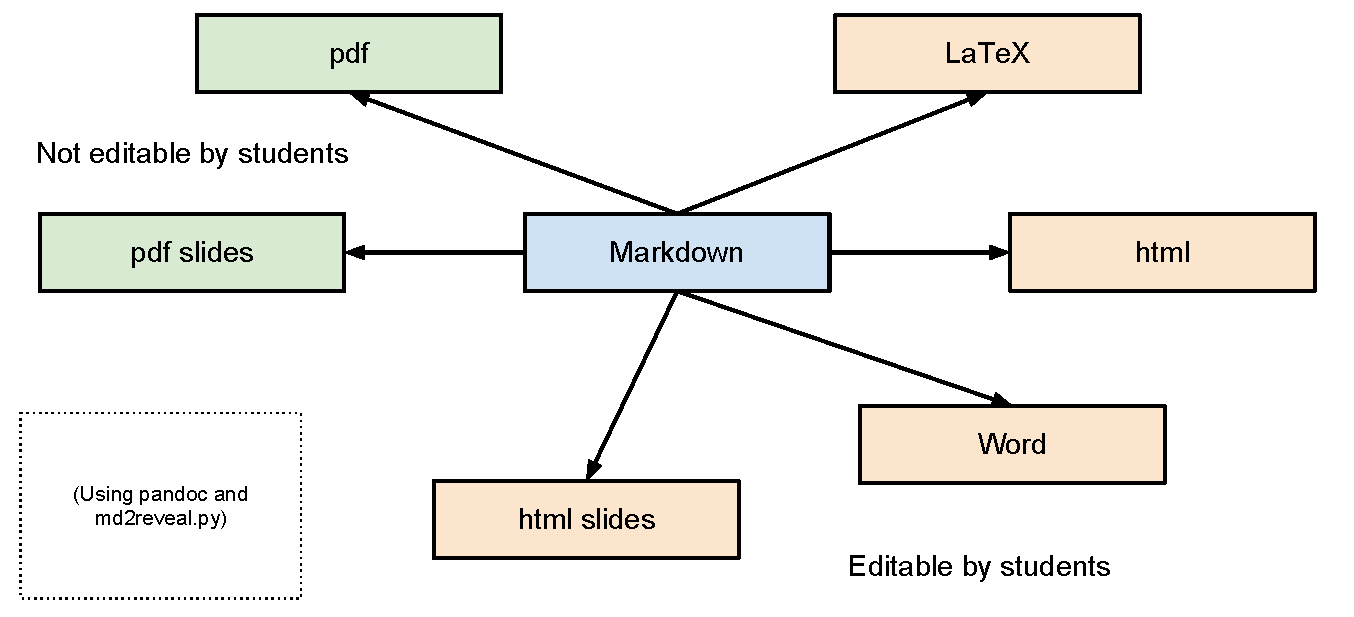
\includegraphics[width=10cm]{Images/using_pandoc.pdf}
    \end{center}
    \caption{Universal formating of materials.}
    \label{using_pandoc}
\end{figure}

Markdown is a very simple language that allows for the rapid creation of teaching materials. Combined with pandoc it can be used to create teaching materials in a variety of formats with little effort. Figure \ref{universal_notes} shows various formats of a document all created from the markdown source.\\

\begin{figure}[htdp]
    \begin{center}
        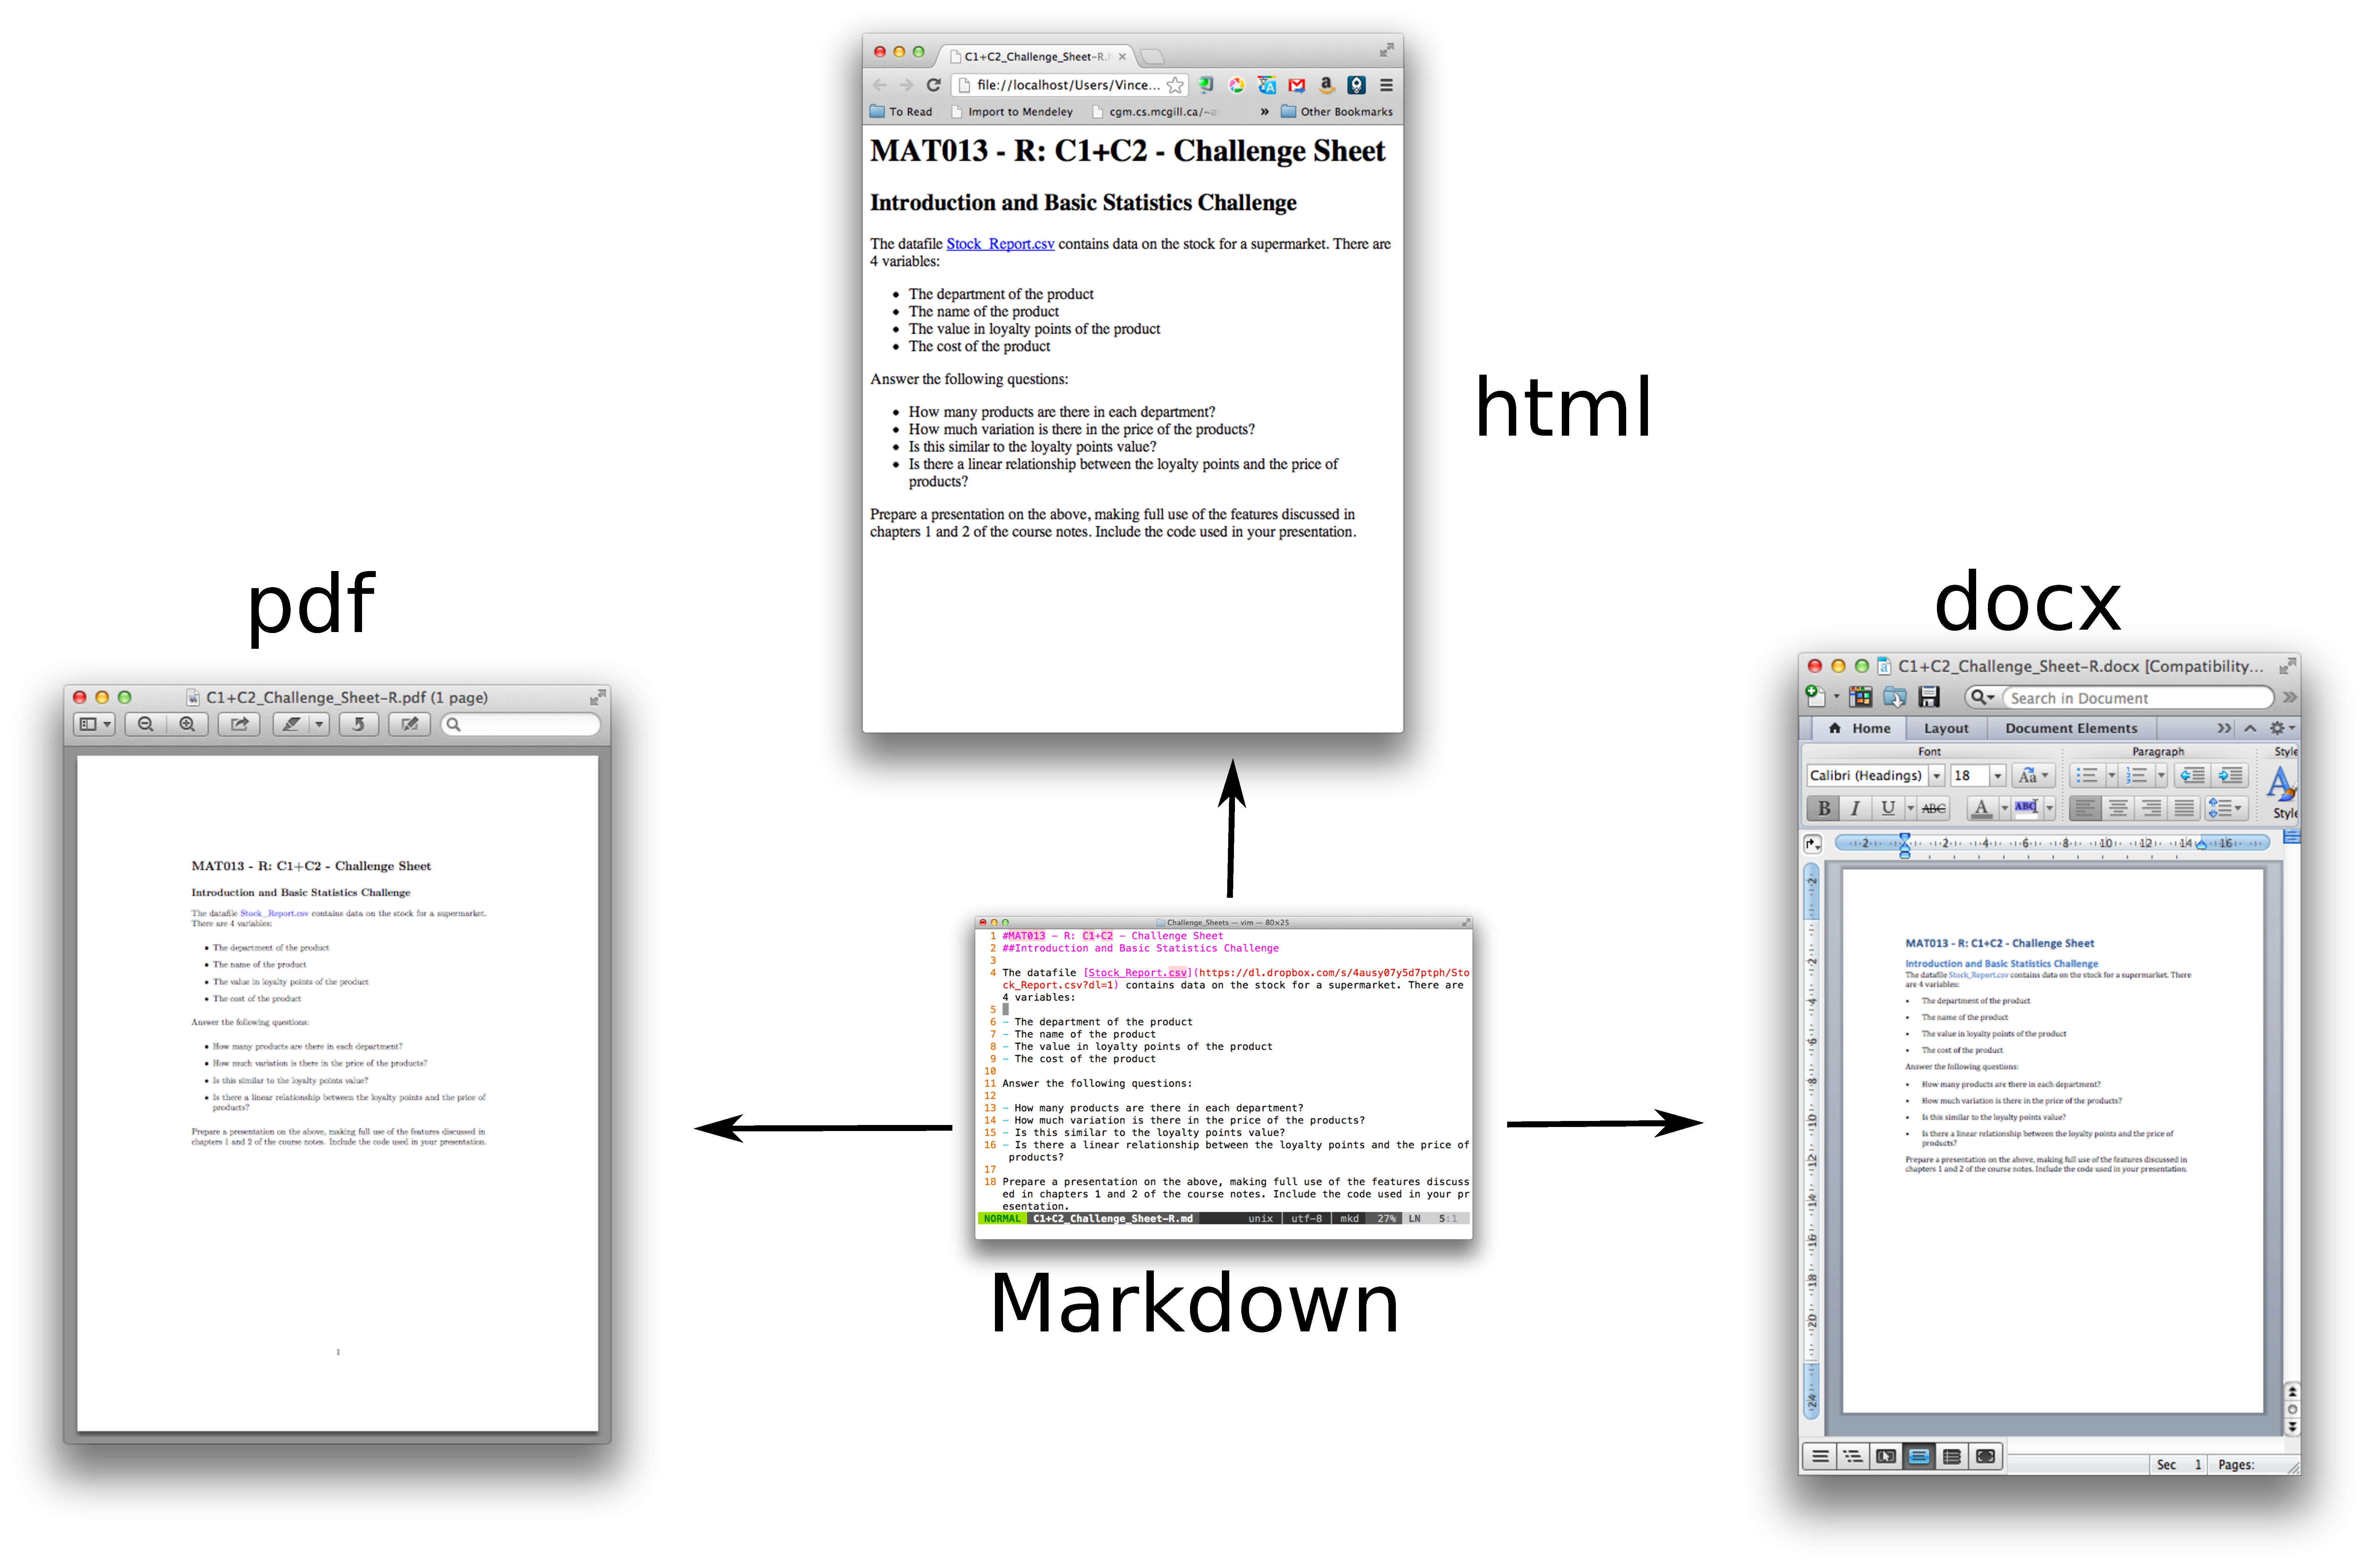
\includegraphics[width=14cm]{images/universal_notes.pdf}
    \end{center}
    \caption{Creating universal notes using pandoc}
    \label{universal_notes}
\end{figure}

I have also created a short programme that makes the creation of these universal notes more efficient. There is an accompanying youtube video available \url{http://www.vincent-knight.com/home/teaching/pcutl}.

From a mathematics point of view an added benefit is that mathematical formulae can also be included.

\section{Informing pedagogy}

I have taken the opportunity to investigate a wide variety of pedagogies through this module. In this section I will discuss a variety of them before describing the particular pedagogy I believe I want to adopt. I obviously understand that I'm at a very early part of my career and my teaching methodologies will surely evolve. Furthermore I am not attempting to find ``the best" pedagogy but more so the pedagogy that is ``best for me". Having said that, in \cite{Kember2007a} a range of award winning teachers are interviewed and it seems that a general set of principles of good teaching can be identified. Here is a quote from \cite{Kember2007a}:

\begin{quote}
    ``The outcomes of the analysis was a set of principles of good teaching practice. Given the diversity of the sample there was a remarkably high degree of consistency to the principles. There was no evidence of any cultural disparity between East and West, indicating perhaps that academics in reputable universities constitute an international culture. The set of principles of good university teaching can, therefore, be seen as having international applicability."
\end{quote}

As such I will now evaluate various pedagogical models in an attempt to identify a good practice of teaching.

\subsection{Philosophy of education}

There are three basic notions of educational philosophy (\cite{Jordan2008a} gives an excellent account of these):

\begin{enumerate}
    \item Ideas
    \item Experience
    \item Development
\end{enumerate}

\textbf{Ideas}: With concepts such as Socratic dialog \cite{Platoa} an emphasis is placed on logic and a questioning of conceptions. In it's essence this is well suited to Mathematics although whether or not ideas relating to the encouraging of discussion of interpretation of ideas is relevant is an interesting question. I asked the question on Google Plus and was quickly answered by a fellow educator (Theron Hitchman from the University of Northern Iowa) who often enters in to a Socratic dialog with his students when using an `Inquiry Based Learning' (IBL) approach \cite{Kember2007a} (including discussions of Theorems), the discussion can be seen here: \url{http://goo.gl/LakrE}.

\begin{quote}
``IBL teaching has a Socratic feel to it, and I find my classes are full of alternate interpretations of everything. common concepts, theorems,... everything. Allowing (requiring?) the students to share and defend their ideas at every meeting has a couple of benefits.

1) you get a better window onto the variety of student misconceptions. Some are quite subtle, and some are so far away from your expectations!

2) students seem to change their minds easier when these subtle errors are pointed out and explained by peers. I think maybe it is partly a `let me down easy' thing, and partly it is that the students will choose more comfortable language to get the point across.

3) If you give them time, and focus your energy on asking questions, each class will eventually come around to the commonly accepted `mathematician's understanding', and they will be much less likely to make that same mistake again. ( not that they won't, but...)"
\end{quote}

I found this short exchange with Theron very worthwhile. It was great to hear that Socratic dialog allowed for the discussion of \emph{Interpretation} of mathematical facts.\\

As stated in \cite{Jordan2008a} the philosophical notion of Idea has 3 main implications for teaching:

\begin{itemize}
    \item an emphasis on theory before practice;
    \item an emphasis on logical thinking;
    \item a high value attached to liberal education.
\end{itemize}

Mathematics is of course very concerned with ideas and concepts and the above comment by Theron Hitchman seems to confirm that a Socratic dialogue is well suited to Mathematics. On the other side of the coin Mathematics is also very concerned with computation and applicability of ideas, this brings us to the next philosophical idea.\\

\textbf{Experience}: This notion is opposed to the previous in that it states that experience is more important than theory. There are two strands in this category:

\begin{itemize}
    \item Empiricism (claiming that students are passive recipients of experience)
    \item Romanticism (claiming that students are actives recipients of experience)
\end{itemize}

The educational implications of empiricism is that learning is a science and has general principles. Sitting well within this idea is Bloom's Taxonomy \cite{Bloom1969a} which specifies different levels of learning as well as how they can be evaluated. In \cite{Shorser1999} Bloom's Taxonomy is mapped on to mathematics, highlighting particular examples and wording for questions that evaluate various levels of learning.\\

The implications of romanticism include that the purpose of education is the development of the whole person and that all learners are different.\\

The final philosophical idea builds on the notion of Experience.\\

\textbf{Development}: This notion compares a teacher to a gardener aiming to grow a plant `to it's full potential'.\\

The corresponding philosophy is `Teleology' which is closely linked to ideas of Aristotle (plants grow, animals, grow and feel, humans, grow feel and think) \cite{Aristotlea}. Unlike the ideas of empiricism which places teachers at the center of the learning experience, this places students at the center of the learning experience.\\

Various implications correspond to this notion including that students must know why they are learning a topic and that they are motivated by goals.\\

\subsection{Learning models}

The three philosophical notions described in the previous section are worth being familiar with when looking at the three following pedagogies which aim to explain how students learn:

\begin{enumerate}
    \item Behaviourism
    \item Cognitivism
    \item Constrictivism
\end{enumerate}

I am purposefully choosing to not discuss other more modern pedagogies (such as `social learning', and/or `cultural learning') as in particular the Social Constructivism of \cite{Vygotsky1978a} seems to encompass them. I will briefly address some of the issues linked to those models in a latter section. How these pedagogies lie within the educational philosophies previously described can be seen in Figure \ref{Learning_Pedagogies}.

\begin{figure}[htdp]
    \begin{center}
        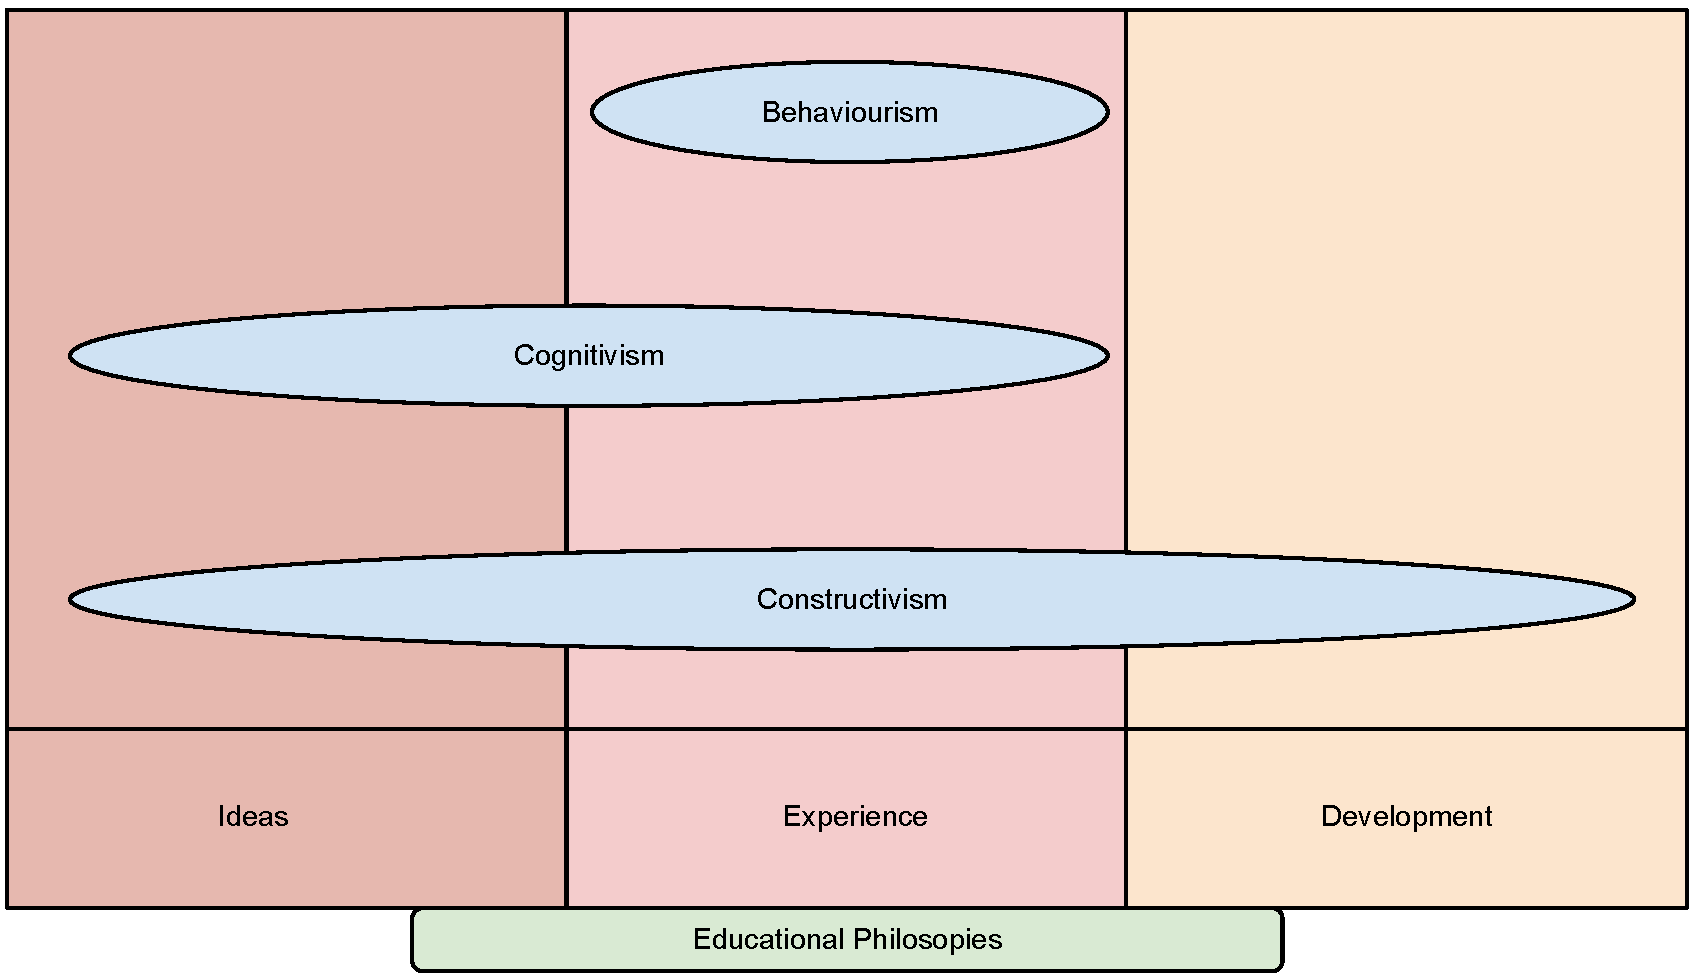
\includegraphics[width=10cm]{Images/Learning_Pedagogies.pdf}
    \end{center}
    \caption{The philosophical basis to some pedagogies.}
    \label{Learning_Pedagogies}
\end{figure}

\subsubsection{Behaviouralism}

Behaviourism relates to classical ideas of conditioning and the early work of Pavlov \cite{Pavlov2003a} which for example showed how to train a dog to salivate when ringing a bell. There are various sub models within behaviourism but the class model is described in \cite{Jordan2008a}:

\begin{quote}
    ``The classical behaviourist view has the stimulus leading directly to the response."
\end{quote}

In \cite{Skinner1961a} teaching machines are described that could potentially put students through a series of stimuli which would let them ``learn''. This notion is perhaps a reality today with the various Massive Open Online Courses (MOOCs) run for example by Coursera (\url{www.coursera.org}) and Udacity (\url{www.udacity.com}) in particular and flipped classrooms in general \cite{Bates,JeremyF.Strayer2007,Mccombs2007}. A further description of MOOCs and other modern teaching approaches can be found in \cite{Sharples2012}.\\

Behaviourism is an efficient pedagogy in promoting rapid learning although it does not promote deep learning (with my experience of MOOCS I can relate to this). Behaviourism also has many negative connotations related to `power and control and has connotations of animal training'.  Behaviourism is a deterministic theory: students are all the same. In general MOOCs attempt to remedy this by encouraging the use of social networks and flipped classrooms aiming to make valuable use of the gained lecture time.\\

\subsubsection{Cognitivism}

The way Cognitivism builds on Behaviourism is nicely explained in a single sentence in \cite{Jordan2008a}:

\begin{quote}
    ``[...] stimulus-response does not explain how children can generate sentences they have not heard before."
\end{quote}

Cognitivism treats students as computers. It assumes that learning is the individual application of a mental process. Cognitivism places education in a technico-rational setting (recall the empiricism philosophy of education). As such it ignores the individualisation of learning by students.\\

\subsubsection{Constructivism}
Finally this leaves us with Constructivism which builds on Cognitivism by understanding not just how a student `perceives' information but also how a student gives the information their own `meaning'.\\

There are various `schools of thought' in constructivism:

\begin{itemize}
    \item `Trivial constructivism': teachers must not interfere with the individual process of reconfiguring perceived information.
    \item  `Social constructivism': teachers should act as a support for the learners thinking. This takes place in the \textbf{Zone of Proximal Development} \cite{Vygotsky1978a}.
    \item  `Critical constructivism': learners should construct `meaning' of information by questioning `hierarchy'. This in essence aims to place teachers as peers.
\end{itemize}

I particularly like the ideas of Vygotsky \cite{Vygotsky1978a} (the father of social Constructvivism) . As an implication to education the idea of Scaffolding appears acting as a support which aims to help learners construct new knowledge.\\

A particular aspect of Social constructivism that I find attractive is that it indeed takes account of the social factor of learning. Social Learning and Cultural Learning are sometimes considered as pedagogic models in their own right yet I feel that for the purposes of teaching Mathematics it is sufficient to consider a Social Constructive model as the ideas of Mathematics are often independent of culture. Indeed, on a personal note, having experience learning in a variety of countries, cultures and as a result: social groups. My liking for Mathematics is not surprising: it was the one subject that did not change as and when I moved from country to country.\\


With regards to Mathematics and my own teaching, reflecting on the feedback analysed in Section \ref{Analysis} the above review of pedagogic models seems to strengthen my observation that student enjoyed and performed well in subjects that were taught in a student lead approach where students are encouraged to discover topics and construct a meaning on their own. This Social Constrivism approach is very similar to IBL approaches \cite{Mahavier2006} and project based learning \cite{Barell2007a,Schwartz2001b}. The IBL approach in general is based on students working through problems alone and presenting them to the class with a high degree of flexibility allowed for students to discover further notions on their own. The quote given at the beginning of this document is by R. L. Moore the father of IBL. As such the lectures are extremely valuable as peer learning takes place, active assessement of student comprehension is always taking place and finally students are always construcing meaning themselves.\\

Note that some themes of this approach can be found in the interviews of award winning teachers, here are certain quotes from \cite{Kember2007a} that I found of value:

\begin{quote}
    ``[...] we established that the award winning teachers believed that teaching was a process of facilitating student learning"
\end{quote}

\begin{quote}
    ``The real learning had taken place when I reflected on the material outside of the lectures, or I read about it or talked about it with colleagues"
\end{quote}

\subsubsection{What teaching pedagogy for me.}

When considering Mathematics, there are various threshold concepts that can be described \cite{Cousin2006,Framework2007,Meyer2003}. In particular the ability to not just carry out a computation but understand the computation is an important one. In \cite{Schoenfeld1988} an account of a particular course that in a traditional sense would be noted as a success is given (for example learning outcomes where achieved). While \cite{Schoenfeld1988} does not describe threshold concepts per say it defines 4 beliefs that are almost the opposite:

\begin{enumerate}
    \item Formal mathematical concepts such as ``proof" has very little to do with ``real world problem solving".
    \item If a student is going to manage a mathematical problem they will do so in less than 5 minutes (implying that if students don't solve a problem in 5 minutes they might as well stop).
    \item Really `getting' mathematics is only doable by geniuses.
    \item Students do well in class by performing tasks and doing well in school (implying that `getting the work done' will do).
\end{enumerate}

Moving away from these beliefs is achieved using a constructivist approach in general and IBL in particular.\\

The issues related to an IBL approach correspond to inclusivity of this approach which might not cater well to students less comfortable with expressing themselves in front of a class. Further problems might arise with the direction of the course as students are encouraged to explore various directions of independently ensuring that intended learning outcomes are achieved could prove problematic.\\

I plan to address this issue by ensuring that all my class content is available to the class prior to the lectures. Indeed, the content will be prepared as if a classic lecture style course was going to be delivered. Further to this, student will also have access to videos of the lecture content: a flipped classroom. The reason behind such an approach is that a flipped classroom will ensure that the required scaffolding as prescribed in classic Vygotskian models \cite{Vygotsky1978a} is in place to ensure a certain direction for the IBL approach.\\

This approach should ensure that students will gain maximal value from contact time, however if content is to be made completely available to students how can I be sure that they will even turn up?\\

This is a common concern about a flipped class methodology but \cite{Bates} gives evidence for the fallacy of this concern:

\begin{quote}
    ``An often-heard comment relating to provision of material to students (usually lecture notes) in advance of class sessions is `If you give them the lecture notes, they might not or won't turn up'. We gave students not just lecture notes, but in effect the entire course content in advance of class sessions: it might reasonably be asked did we not have empty lecture theatres by week 5? In fact, we did not see any evidence of a significant decline in lecture attendance 1, which we were able to `measure' by observing a relatively constant number of total clicker votes per question (across 140 individual clicker question episodes) as function of a time period spanning 11 weeks of the course. There was a slight decline towards the final week of teaching in the semester, perhaps partly explained by the effects of a long teaching semester taking its toll and the looming shadow of degree examinations 2 weeks after the course concludes. This teaching methodology, therefore, provides evidence against the `no notes in advance' argument as a technique to maintain student attendance and engagement.''
\end{quote}

Further to this in \cite{Bates} a detailed account is given as to the effectiveness of a flipped classroom approach as far as learning is concerned which I feel further evidences the effectiveness of this approach for Mathematics. As shown in Figure \ref{flipped_classroom} the delivery of content which is often quite intense in a classic Mathematics lecture can take place independently to ensure that comprehension and construction of meaning can take place with the help of a lecturer.\\

\begin{figure}[htdp]
    \begin{center}
        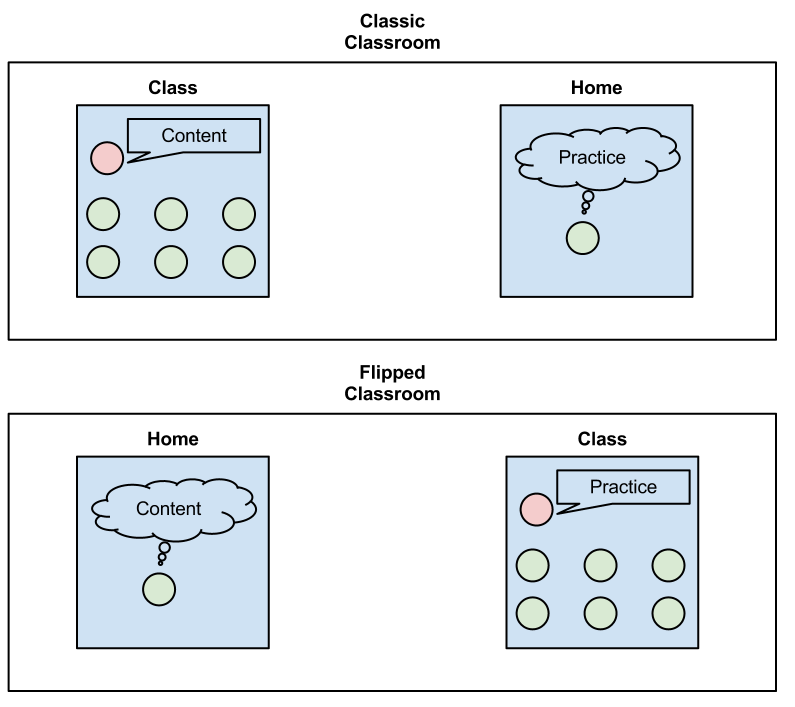
\includegraphics[width=10cm]{Images/flipped_classroom_diagram.png}
    \end{center}
    \caption{A diagrammatic explenation of a flipped classroom.}
    \label{flipped_classroom}
\end{figure}

A potential negative aspect to a flipped classroom is non-engagement of students, to ensure that this is not a concern, the IBL aproach will encourage students to present, explain, and work on solutions to various challenges that I shall present to them. As such it is hoped that construction of meaning will also take place outside of the class and activities in the class will ensure peer learning and further scaffolding to ensure that all ILOs are met.\\

I feel that placing myself as a Social Constructivist with a hybrid IBL/flipped classroom approach will fully enable me to take advantage of both models whilst avoiding the potential negatives. As noted in \cite{Kember2007a} the use of technology in particular and flipped classrooms in general sit well in a Constructivist framework. Furthermore an IBL approach and the corresponding socratic dialogs surrounding student presentations sit very well in the ZPD of Vygotskyan models.\\

Returning again to the feedback discussed in Section \ref{Analysis} I feel that investing myself fully in this approach will improve the learning experience of my students.\\

In an upcoming course (the lesson plans of which have been peer reviewed for this portfolio), I have decided to use this approach. A talk I've prepared explaining the slightly unorthodox methodology can be found in the documentations accompanying my lesson plan.\\

\subsection{Consider social and cultural learning}

In Figure \ref{Learning_Pedagogies} and in my previous discussion I have purposefully ignored certain learning models concerned with the group interactions related to student learning \cite{Jordan2008a}:

\begin{itemize}
    \item Social Learning
    \item Cultural Learning
\end{itemize}

These two models are concerned with the placement of a learner within a group setting and the impact of the group on learning. The first states that `learning does not occur in isolation; it is socially constructed' whilst the second is interested with concepts more closely linked to inclusivity saying that `students' cultural perspectives influence how they construct knowledge' \cite{Jordan2008a}.\\

Initially the IBL aspect of my proposed teaching approach should ensure that learning does not take part in isolation for my students, however due to certain cultural aspects in a multi-cultural class it might prove difficult for students to engage fully. To remedy this I plan to encourage group work as much as possible in my teaching. Groups will be constructed in a way as to ensure that students are able to fully reach their potential.\\

As such I will also look at using virtual communities. There are various papers that look at the use of discussion boards and/or social media in teaching \cite{Gannod2012,Horstmanshof}. There are various benefits to this: in \cite{Junco2011} it is in fact shown that engagement with twitter improved students' marks.  As highlighted in \cite{Wilkinson2011} there are various pitfalls, to avoid these I plan on using a Google Plus community. In \cite{Gannod2012} various social networks are analysed and an advantage seems to be allocated to Google Plus due to it's versatility, interestingly the paper was written prior to `communities' being made available. I believe that communities will allow for students to interact and peer learn. Importantly students do not need to join Google Plus to use it, this in itself (from a technological point of view) is a strength.

\section{Building and participating in learning communities}

I have participated and contributed in many ways to learning communities:

\begin{itemize}
    \item Participated in discussions on the PCUTL discussion boards;
    \item Participated in various discussions on social media on the subject
    \item Blogged reviewing various pieces of educational literature;
    \item Participated in an HEA meeting looking at the teaching of programming in Mathmatics programs.
\end{itemize}

\subsection{PCUTL Discussion board}

I participated in various ways with the PCUTL discussion board. Figure \ref{Lesson_plan_1} shows a screenshot of my Module 1 lesson plan on the discussion board.\\

\begin{figure}[htdp]
    \begin{center}
        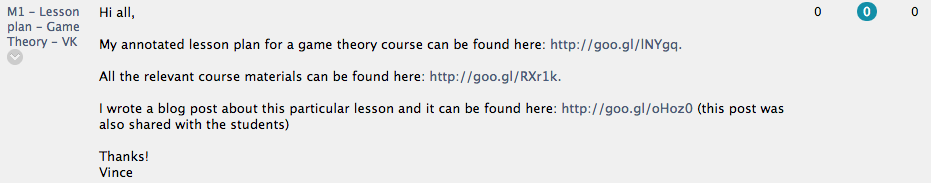
\includegraphics[width=10cm]{./images/Lesson_plan_1}
    \end{center}
    \caption{My Module 1 lesson plan on the PCUTL discussion board}
    \label{Lesson_plan_1}
\end{figure}

Figure \ref{Lesson_plan_2} shows a screenshot of my Module 2 lesson plan on the discussion board.\\

\begin{figure}[htdp]
    \begin{center}
        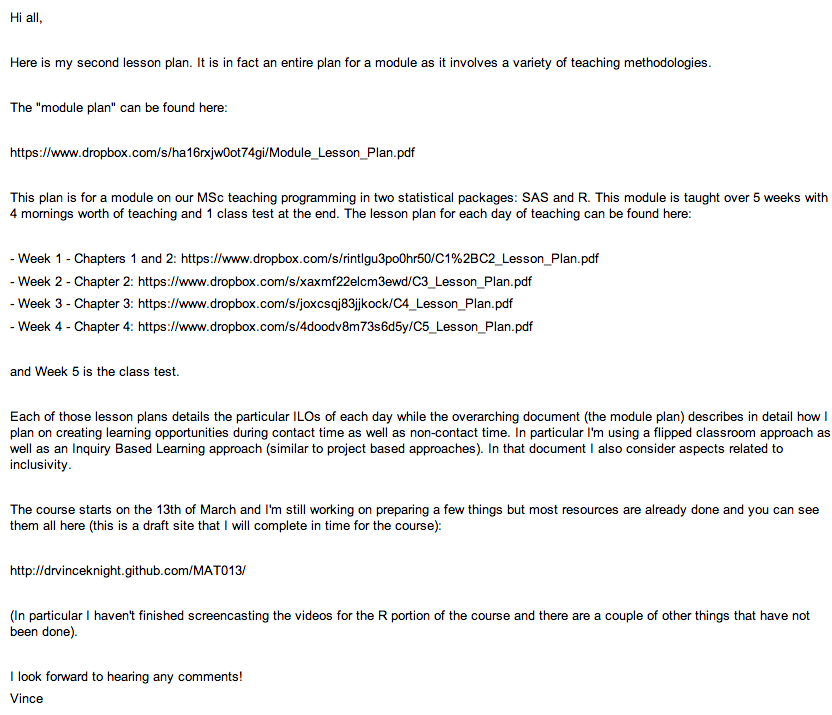
\includegraphics[width=10cm]{./images/Lesson_plan_2}
    \end{center}
    \caption{My Module 2 lesson plan on the PCUTL discussion board}
    \label{Lesson_plan_2}
\end{figure}

One of my early posts on the discussion board was some links to a free book available online discussing various pedagogic models as see in Figure \ref{free_book}.\\

\begin{figure}[htdp]
    \begin{center}
        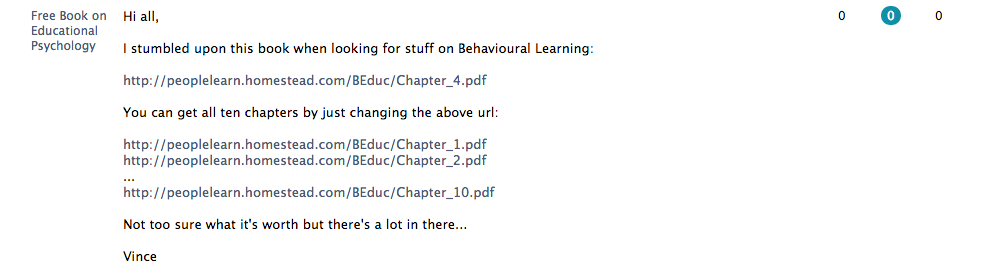
\includegraphics[width=10cm]{./images/free_book}
    \end{center}
    \caption{Sharing a book on the PCUTL discussion board}
    \label{free_book}
\end{figure}

I also entered in to various conversations with my peers including a discussion on the subject of discussion boards itself. Figure \ref{Discussion_board} shows some of the discussion.\\

\begin{figure}[htdp]
    \begin{center}
        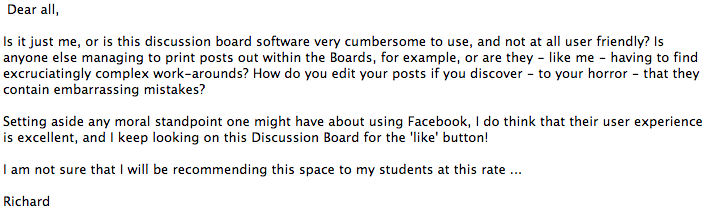
\includegraphics[width=10cm]{./images/Discussion_board-a}
        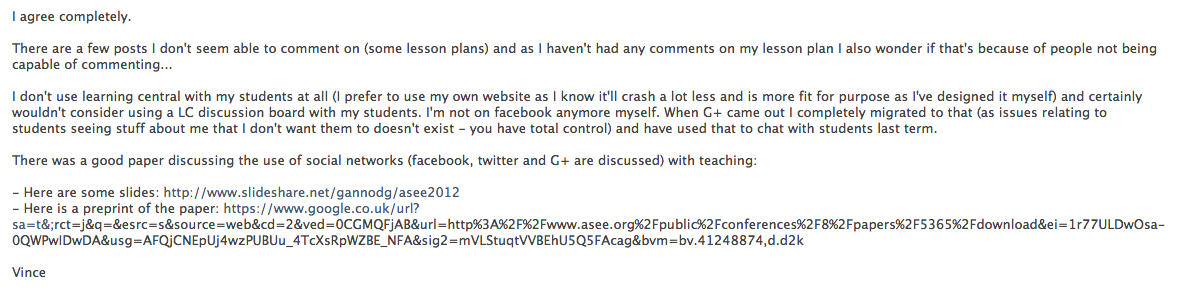
\includegraphics[width=10cm]{./images/Discussion_board-b}
        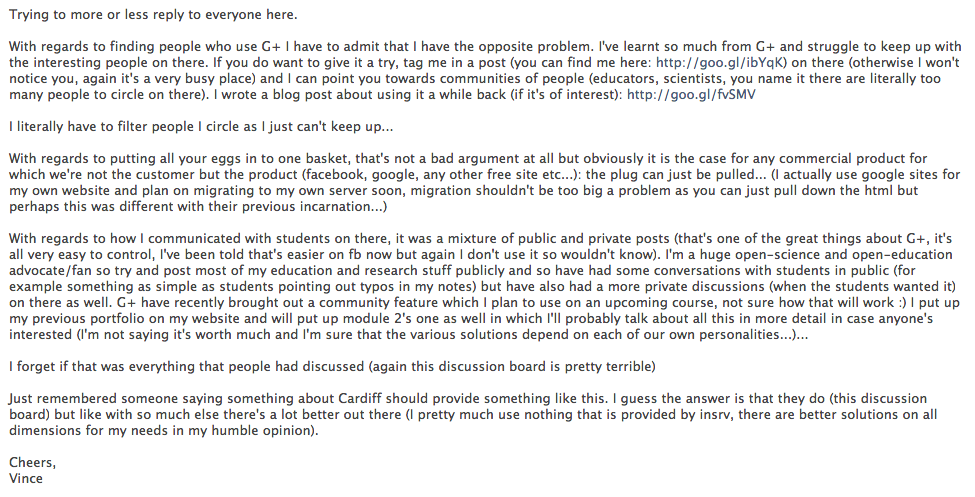
\includegraphics[width=10cm]{./images/Discussion_board-c}
    \end{center}
    \caption{Discussing discussion boards on the PCUTL discussion board}
    \label{Discussion_board}
\end{figure}

I also gave some feedback with regards to some of my peers lesson plans as shown in Figures \ref{chat_with_richard} and \ref{chat_about_jeremys_M2_lesson_plan}.\\

\begin{figure}[htdp]
    \begin{center}
        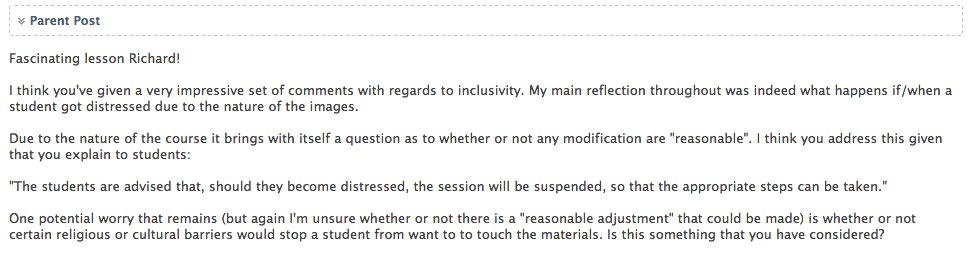
\includegraphics[width=10cm]{./images/chat_with_richard-a}
        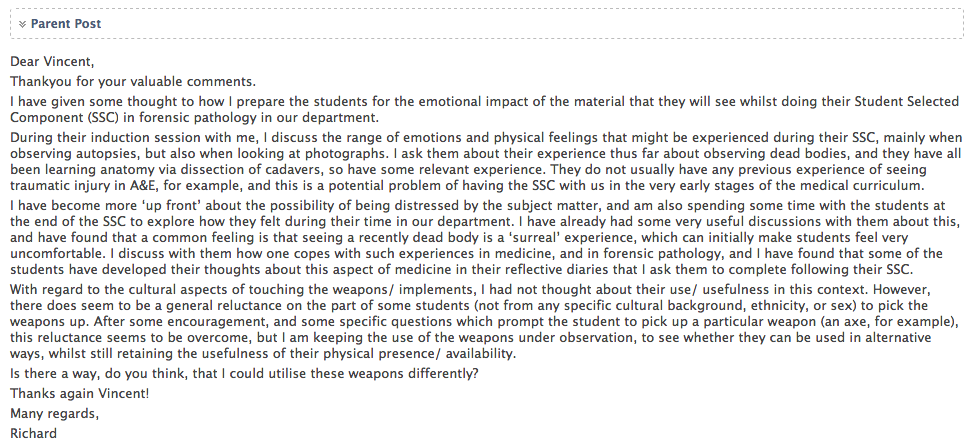
\includegraphics[width=10cm]{./images/chat_with_richard-b}
        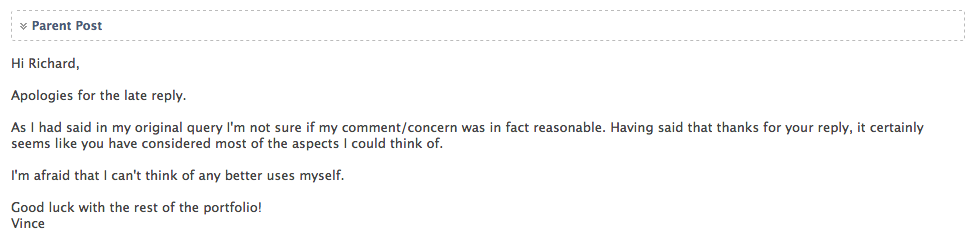
\includegraphics[width=10cm]{./images/chat_with_richard-c}
    \end{center}
    \caption{Discussing inclusivity in a forensic medecine lesson plan}
    \label{chat_with_richard}
\end{figure}

\begin{figure}[htdp]
    \begin{center}
        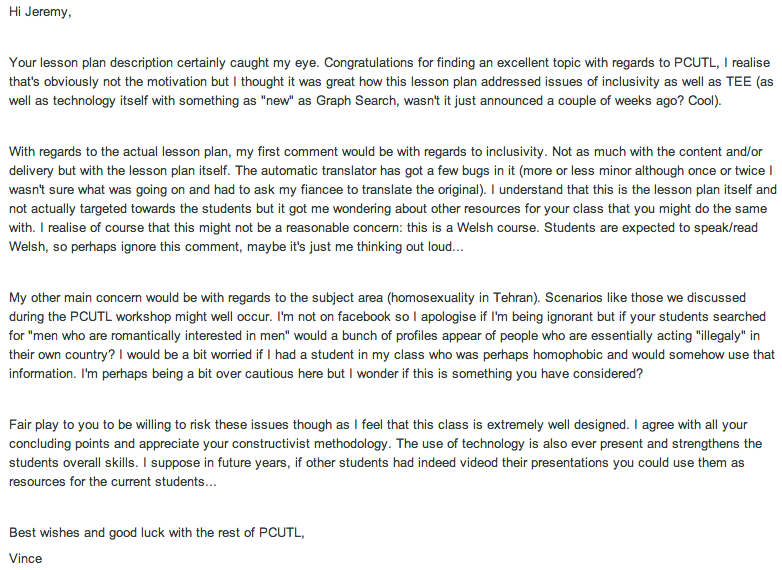
\includegraphics[width=10cm]{./images/chat_about_jeremys_M2_lesson_plan}
    \end{center}
    \caption{Discussing certain issues of inclusivity in a Welsh lesson plan}
    \label{chat_about_jeremys_M2_lesson_plan}
\end{figure}

Due to my interests in flipped classrooms I also shared some resources on flipped classrooms on the PCUTL discussion board as shown in Figure \ref{flipped_classrooms}.\\

\begin{figure}[htdp]
    \begin{center}
        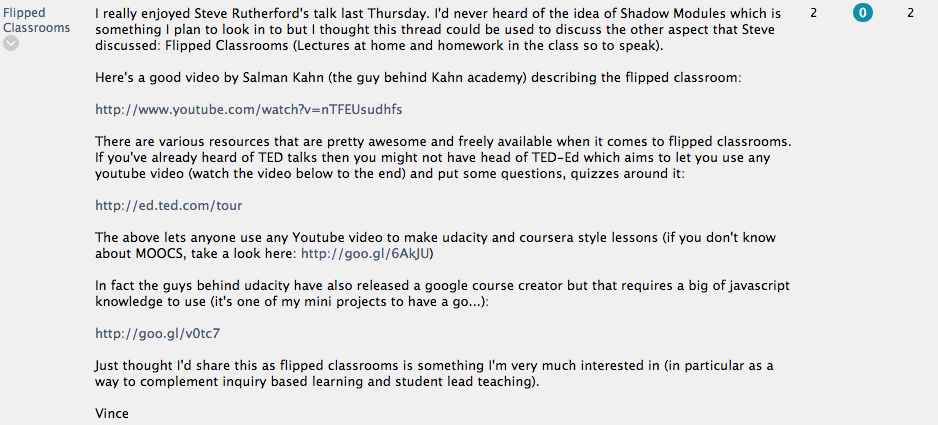
\includegraphics[width=10cm]{./images/flipped_classrooms}
    \end{center}
    \caption{Sharing flipped classroom resources on the PCUTL discussion board}
    \label{flipped_classrooms}
\end{figure}

This led to a further communication with a PCUTL peer on the discussion board as shown in Figure \ref{chat_with_jeremy}.\\

\begin{figure}[htdp]
    \begin{center}
        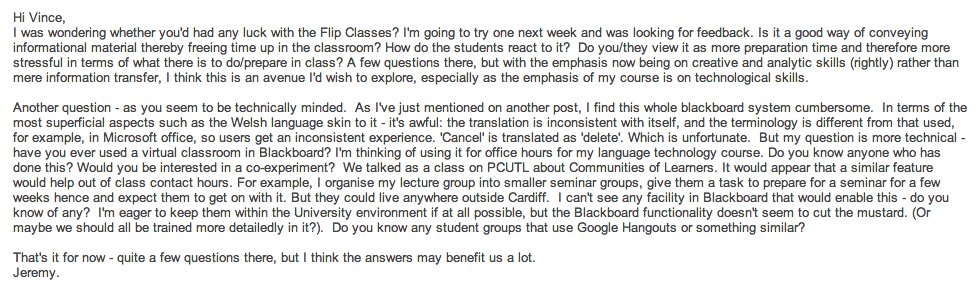
\includegraphics[width=10cm]{./images/chat_with_jeremy-a}
        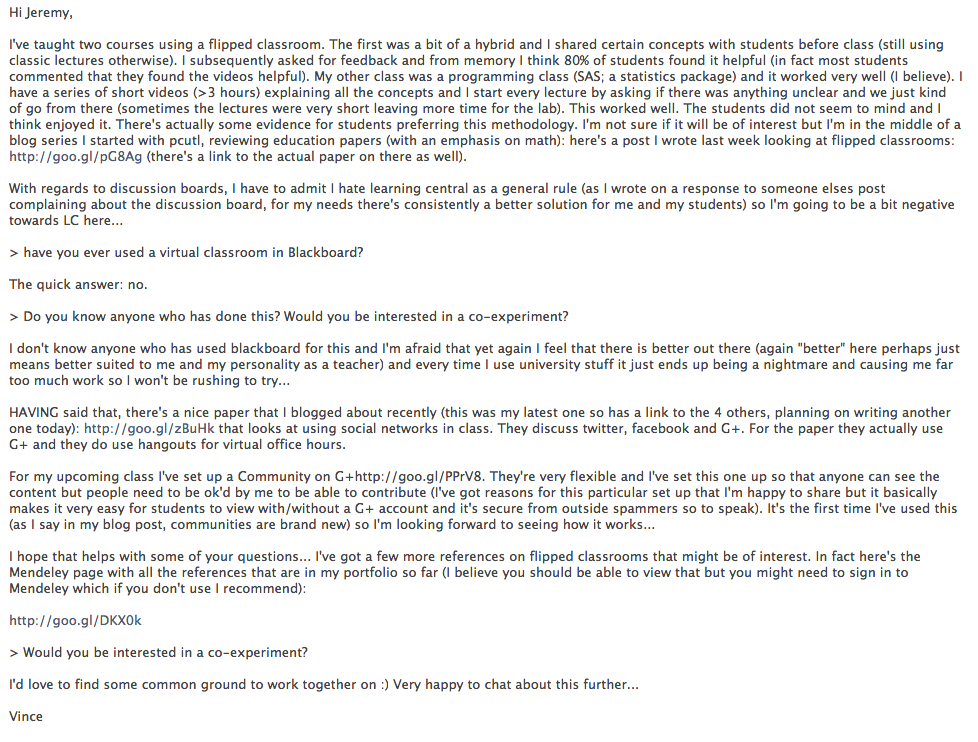
\includegraphics[width=10cm]{./images/chat_with_jeremy-b}
    \end{center}
    \caption{Chatting with Jeremy Ewas on the PCUTL discussion board}
    \label{chat_with_jeremy}
\end{figure}

Whilst I found this process quite rewarding and the exchange of concerns and resources with my peers interesting I think that the technical platform used (as I discussed on the discussion board itself) is quite outdated and does not facilitate an easy transfer of communication. Before starting PCUTL I already made quite a big use of social media. In the next section I will give certain examples of some of the great interactions I have had with fellow teachers.\\

\subsection{Use of Social Media}

My social network of choice is Google Plus. There are various reasons for my choice of social platform but do not feel that it is worth explaining them here (I have written a blog post describing my experiences of using Google Plus as an academic: \url{http://goo.gl/fvSMV}).\\

I have found certain resources for this very portfolio on Google Plus as shown in Figure \ref{finding_paper_on_G+}.\\

\begin{figure}[htdp]
    \begin{center}
        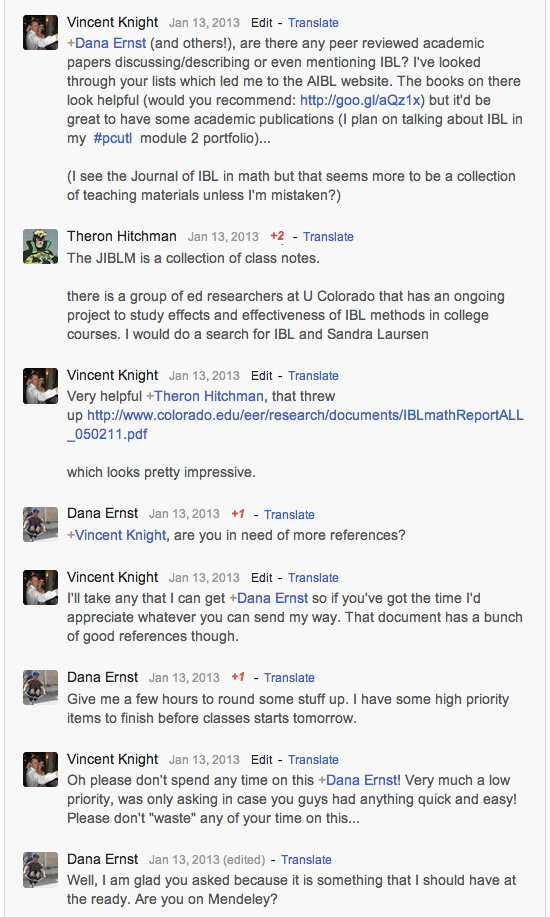
\includegraphics[width=5cm]{images/finding_paper_on_G+.png}
    \end{center}
    \caption{Finding educational resources on Google Plus}
    \label{finding_paper_on_G+}
\end{figure}

I've had discussions discussing teaching approaches as shown in Figure \ref{chat_about_teaching_resources}.\\

\begin{figure}[htdp]
    \begin{center}
        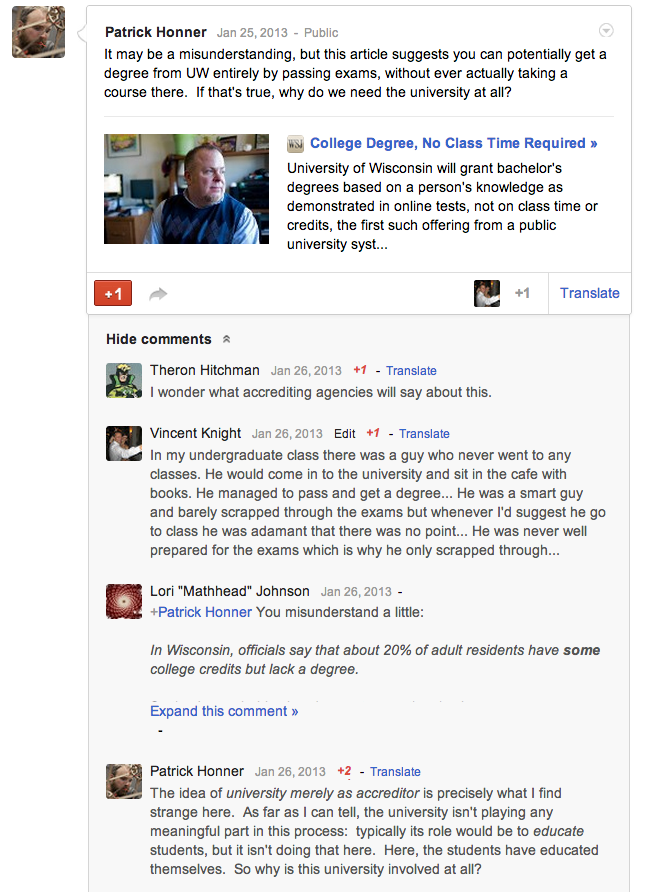
\includegraphics[width=5cm]{images/chat_about_teachers-a.png}
        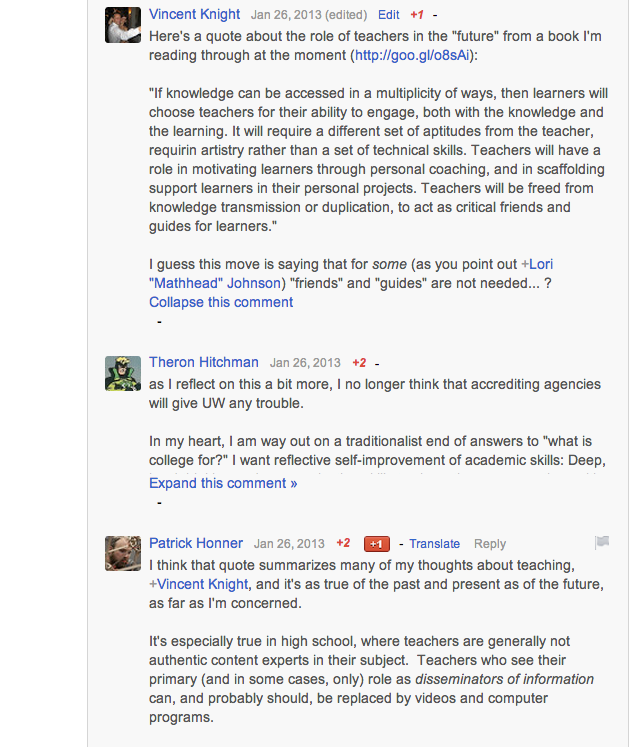
\includegraphics[width=5cm]{images/chat_about_teachers-b.png}
    \end{center}
    \caption{Discussing good teaching}
    \label{chat_about_teaching_resources}
\end{figure}

I've also had some very useful pointers and discussions of my own teaching resources as shown in Figure \ref{chat_about_Shapley_value_video}.\\

\begin{figure}[htdp]
    \begin{center}
        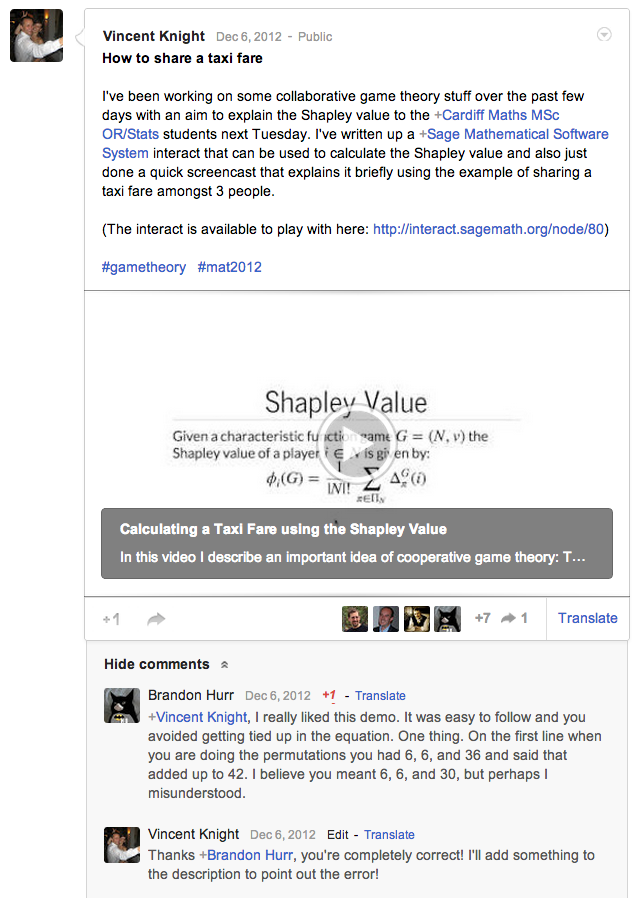
\includegraphics[width=5cm]{images/chat_about_Shapley_value_video.png}
    \end{center}
    \caption{Sharing a video on the Shapley value}
    \label{chat_about_Shapley_value_video}
\end{figure}

I've shared `circles' of educators as shown in Figure \ref{Sharing_my_education_circle}.\\

\begin{figure}[htdp]
    \begin{center}
        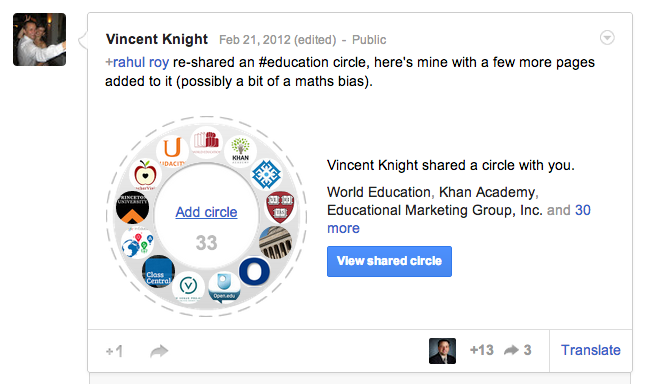
\includegraphics[width=10cm]{images/Sharing_my_education_circle.png}
    \end{center}
    \caption{Sharing a community of educators}
    \label{Sharing_my_education_circle}
\end{figure}

Finally, as discussed previously, I have used and continue to use Google Plus with my students encouraging them to not online interact amongst each other but also to engage with various teachers and practitioners in the field of Mathematics in general and Operational Research in particular.\\

\subsection{Educational Literature Review}

As well as using Social media I also have a blog that I use to post about my teaching and research (for example here is the blog post related to the class I taught for my peer reviewing module 1: \url{http://goo.gl/oHoz0}).\\

For this module of PCUTL as I made it a point to read a lot of education literature I decided to blog short reviews of as many pieces of literature as I found time to do. A list of these posts with links to each one is available at \url{www.vincent-knight.com/teaching/pcutl}.\\

The blogs posts were quite well received:

\begin{itemize}
    \item Currently more than 700 views
    \item Most viewed post was my first one (currently 136 views and one short interesting conversation) which reviewed \cite{Schoenfeld1988}.
    \item Least viewed post (currently only 48 views) which reviewed \cite{Shorser1999}.
\end{itemize}

I received some warm comments on social media. Here is a quote from a teaching in the USA who I was thanking for sharing one of my posts on Twitter to his 2049 followers.

\begin{quote}
    ``My pleasure--I'm enjoying recent focus on math ed issues.  I think a lot about learning and teaching, but I wouldn't say I'm extremely well-read on the topics.  It's nice to following along with what you're reading, as well as have another voice in the conversation!''
\end{quote}

\subsection{HEA Meeting on programming}

In the next academic year I will be teaching a new first year module aiming to teach computer programming for Mathematics. With this in mind on the 4th of February 2013 I went to a one day HEA workshop entitled: `HEA STEM (Maths, Stats and OR): Experiences of learning programming within a Mathematics course'.\\

There were 20 delegates present from universities all of the UK. It was a great networking opportunity and I was able to learn quite a few things from the experiences of other teachers which I will take forward in the preparation on of a module I'm teaching next academic year.\\

\section{Further development}

There are various dimensions in which I can expand my professional development as a teacher:

\begin{itemize}
    \item Further understanding of pedagogic models;
    \item Further understanding of methodologies;
    \item Further building and participating in learning communities.
\end{itemize}

On a very tangible note however, an immediate issue that I aim to evaluate is the marking of group projects. There is a growing body of literature aiming to inform best practice when it comes to recognizing individual performance in group work \cite{Lejk1996a}.\\

As I plan to use a lot of group work in my teaching I feel that this is something I need to look at closely. An initial investigation of the literature \cite{Lejk1996a,Kember2007a} shows that most approaches make use of feedback from students to evaluate the individual contribution of all group members. I do not see any alternative to this approach but do believe that a more sophisticated and fair approach could be used to map perceived contributions to marks.\\

Following discussions with my mentor Professor Paul Harper, the approach we propose would place group work within a cooperative game theoretic framework and would use the Shapley value to fairly recognise individual contributions. The Shapley value can be calculated using the following equation (I realise that this is given in this document without sufficient explication):

\begin{equation}
    \phi_i(G)=\frac{1}{|N|!}\sum_{\pi\in\Pi_N}\Delta_{\pi}^{G}(i)\label{Shapley_def}
\end{equation}

There are issues of transparency that must be overcome when using such an approach but in a Mathematics department these should not be insurmountable. The idea revolves around the potential contributions of all subgroups within a group. Consider the following feedback obtained from a group of three students ascertaining what potential of the total mark would have been obtained by each subgroup of the group:

\begin{center}
    \begin{tabular}{c|c}
        $S$&$v(S)$\\
        \hline
        $A$&40\\
        $B$&40\\
        $C$&20\\
        $\{A,B\}$&70\\
        $\{A,C\}$&60\\
        $\{B,C\}$&40\\
        $\{A,B,C\}$&100
    \end{tabular}
\end{center}

Using equation (\ref{Shapley_def}) the Shapley value can be calculated for each member of the group:

\begin{center}
    \begin{tabular}{c|c}
        Student&$\Phi$\\\hline
        $A$&45\\
        $B$&35\\
        $C$&20
    \end{tabular}
\end{center}

If we assume that the marking criteria states that group work would be marked with 70\% of the mark being dependant on output and 30\% being dependent on group work a fair mark could be given using the following formula:

\begin{equation}
    m(i)=M\times\left(.7+.3\times\frac{\Phi(i)}{\max_{j}\Phi(j)}\right)
\end{equation}

Where $M$ is the total mark given to the project. In our above example, if we assume that the project was worth 85 the marks given to each individual would be:


\begin{center}
    \begin{tabular}{c|c}
        Student&Mark\\\hline
        $A$&85\\
        $B$&78\\
        $C$&71
    \end{tabular}
\end{center}

As discussed this approach still needs to be carefully considered. One of the immediate disadvantages of this approach is it's transparency. Various resources would need to be put in place to ensure that students \emph{understood} the approach. As described previously I feel that in a Mathematics department this is not unsurmountable. Furthermore, there are various advantages to this approach. First of all, it is theoretically sound and is in fact the only `fair' approach of distributing marks. Various other aspects are advantages to this approach such as the fact that the only way for students to maximise their marks is for them all to contribute equally.\\

Further investigation of this approach is an exciting prospect as I feel it would be of publishable quality in a reputable education journal.

\newpage
\bibliographystyle{plain}
\bibliography{mathed.bib}

\end{document}
